% Copyright 2022  李文威 (Wen-Wei Li).
% Permission is granted to copy, distribute and/or modify this
% document under the terms of the Creative Commons
% Attribution 4.0 International (CC BY 4.0)
% http://creativecommons.org/licenses/by/4.0/

% 《代数学方法》卷一自订封面页, 由主档引入.

\setCJKfamilyfont{coverfont}{Noto Serif CJK SC Bold}	% 设置书名字体
\setCJKfamilyfont{cover-author-font}{Noto Sans CJK SC}	% 设置作者字体
\colorlet{octa}{cyan!50!gray}	% Color for the octahedron

\begin{titlepage}
\begin{figure*}
\begin{tikzpicture}[remember picture, overlay, pencildraw/.style={
		color=octa, thick,
		decorate,
		decoration={random steps, segment length=1pt, amplitude=0.7pt}
	}]

	\node[anchor=center] (title) at ([xshift=19em, yshift=-10em] current page.north west)
		{ \fontsize{45}{45}\CJKfamily{coverfont} Infinite Categories};

	\node[anchor=center] (volume) at ([yshift=-7em, xshift=30pt] title.center) {\fontsize{30}{30}\CJKfamily{coverfont}无穷范畴};

	\node[anchor=west] (author) at ([yshift=-5em, xshift=9pt] volume.south west) {\fontsize{18}{18}\CJKfamily{cover-author-font}\kaishu{刘欧}};
	\node[anchor=west] at ([xshift=2.4em] author.east) {\fontsize{18}{18}\CJKfamily{cover-author-font}};

	\draw[line width=2pt, color=black!70!gray] ([xshift=-2.5em, yshift=1em] author.north west) -- ++(25em,0);
	\shade[top color=gray, bottom color=black,] ([xshift=-1em, yshift=1em] title.north west) rectangle ++(-1em,-20em);

	% The anchors for the pictures at lower-right corner.


\end{tikzpicture}
\end{figure*}
\begin{figure*}
    \vspace{7cm}
    \centering
    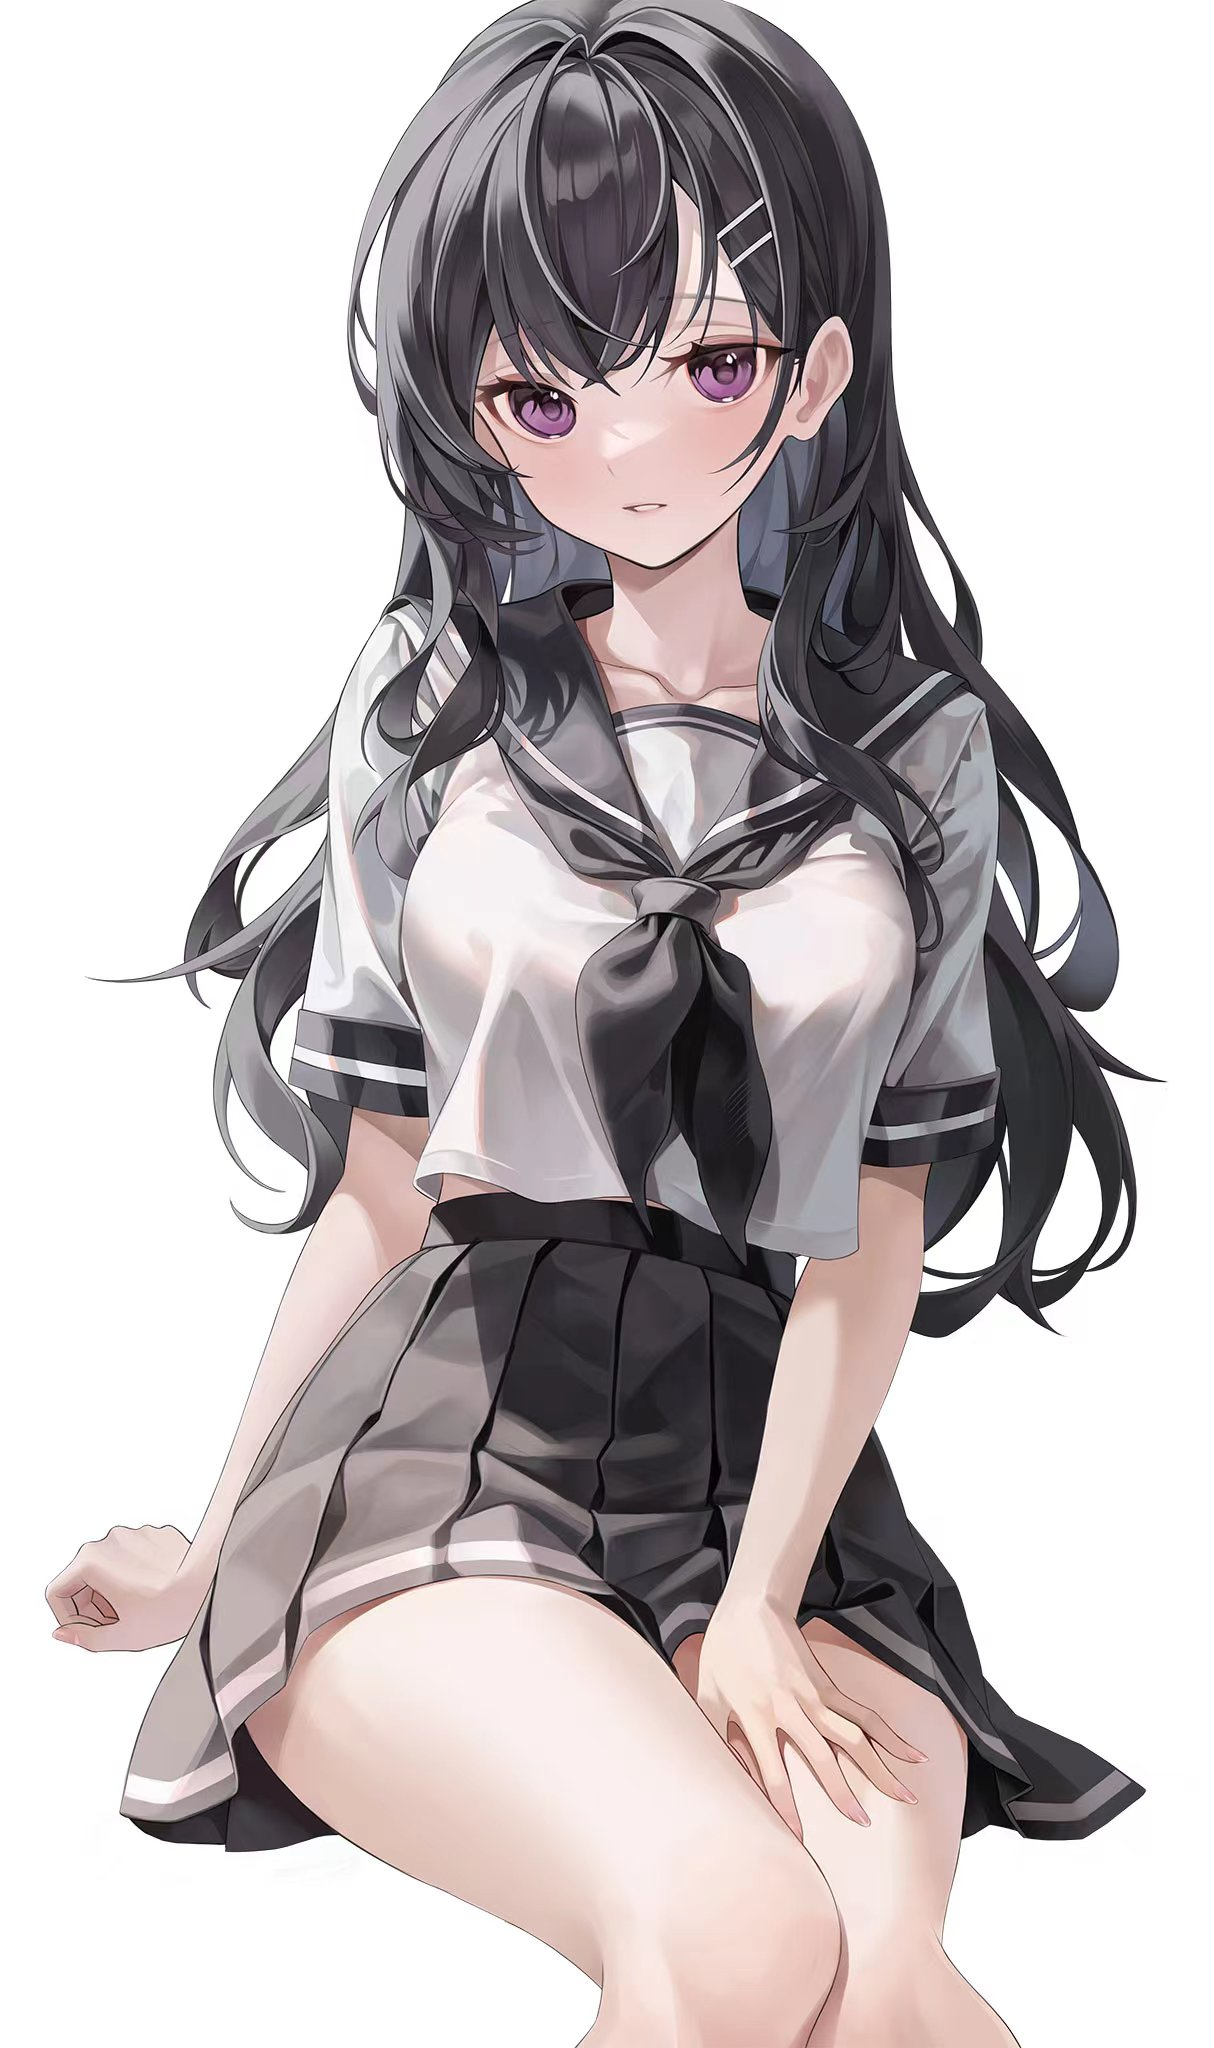
\includegraphics[width=0.5\linewidth]{封面.jpg}
\end{figure*}
\clearpage	% 进入内页
\begin{center}
	\Large{\sffamily\bfseries\thmheiti 内测版  \\  2024年6月21日起编写 } \\ \vspace{2em}
	\Large{\sffamily\bfseries\thmheiti 编译日期: \today} \\ \vspace{1em}
%	版面: B5 (176×250mm) \\ \vspace{1em}
\end{center}
\vfill

\begin{flushleft} \small
	山西大学基础数学讨论班 \\
	群聊:598842179 \\
        沿用李文威.代数学方法所使用模板,主页: \href{https://www.wwli.asia}{www.wwli.asia}\\
\end{flushleft}
\vspace{1.5em}


\cleardoublepage
\end{titlepage}
